\chapter{Quickstart}

\section{Startup}
\label{sec:startup}
Run from the command line without arguments, \progname{} starts up with the full GUI. If model files are given as arguments these are all loaded in to Aten, provided they are of a compatible format. Whether a model file is readable and/or writable by \progname{} is determined by the current stock of filters available to the program (see \ref{sec:filters}). These are read from the location pointed to by \$ATENDATA and, if found, from \$HOME/.aten/filters. In addition, a user preferences file named \qte{prefs.dat} may exist in \$HOME/.aten and control many aspects of the program (in fact, the preferences file is treated as a script file -- see \ref{sec:scripts}).\\

Many command-line options exist to allow for immediate loading of models, scripts, forcefields etc., and to run the program in batch mode etc. See Section \ref{sec:cli} for a full list.\\

\section{Main Window}
Most of the main window is taken up with a canvas which is used to display and edit models and take input from the user. Each of the mouse buttons has a different action on the canvas, each of which can be set to the users taste in the preferences (menu item Settings$\rightarrow$Preferences on Linux). In addition the Shift, Ctrl, and Alt keys modify or augment these default actions. See the following sections for brief descriptions of the different modes. At the foot of the window is a message box (where output and errors are thrown) and a status bar reflecting the content of the current model displayed, listing the number of atoms and the number of selected atoms (bold value in parentheses, but only if there are selected atoms), the mass of the model, and the cell type and density of the model (if it is periodic).\\

A stack of icons on the right-hand side of the window provides quick access to different tool panels for building, analysing etc. The icons are:\\

\noindent
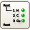
\includegraphics[width=1cm]{images/stack_atomlist} Shows a list of atoms in the model \\

\includegraphics[width=1cm]{images/stack_cell} Add, edit, or transform the model's unit cell \\

\includegraphics[width=1cm]{images/stack_edit} Tools to edit atoms and bonds \\

\includegraphics[width=1cm]{images/stack_transform} Transform selections of atoms \\
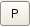
\includegraphics[width=1cm]{images/stack_position} Position selections of atoms \\

\includegraphics[width=1cm]{images/stack_ff} Load and edit forcefields, and assign to models and patterns \\
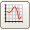
\includegraphics[width=1cm]{images/stack_minimise} Minimise the energy of models \\

\includegraphics[width=1cm]{images/stack_disorder} Create disordered systems \\

See the relevant sections of the manual for descriptions of each of these panels.

\section{Changing the View}
At its most basic the canvas acts as a visualiser allowing models to be rotated, zoomed in and out, and drawn in various different styles. By default, the right mouse button is used to rotate the molecule in the plane of the screen (right-click and hold on an empty area of the canvas and move the mouse to rotate the model) and the mouse wheel zooms in and out. Note that right-clicking on an atom brings up the atom menu (see Section \ref{sec:atommenu}). The middle mouse button translates the model in the plane of the screen -- again, click-hold and drag. Rotation and translation operate on the position and orientation of the camera and no modifications to the actual coordinates of the model are made. The view can be reset at any time from the main menu (View$\rightarrow$Reset) or by pressing Ctrl-R. Both the main menu (View$\rightarrow$Style) and the View toolbar allow the drawing style of models to be changed between stick, tube, sphere, scaled sphere, and individual. The last option allows different view styles to be set for different atoms.\\

The Ctrl key changes the normal behaviour of the rotation and translation operations and forces them to be performed on the coordinates of the current atom selection instead of the camera. The centre of rotation is the geometric centre of the selected atoms.

\section{Selection}
Atom selection or picking is performed with the left mouse button by default -- single-click on any atom to highlight (select) it. Single-clicks perform \qte{exclusive} selections; that is, all other atom(s) are deselected before the clicked atom is (re)selected. Clicking in an empty region of the canvas deselects all atoms. Clicking on an empty space in the canvas, holding, and dragging draws a rectangular selection region -- releasing the mouse button then selects all atoms within this area. Again, this selection operation is exclusive. Inclusive selections (where already-selected atoms are not deselected) are performed by holding the Shift key. Furthermore, single-clicking on a selected atom while holding Shift will deselect the atom.\\


To summarise mouse control, out of the box the standard settings are:\\

\begin{table}[h!]
  \caption{}
  \begin{tabular}{cc|l}
\hline
	Button	& Modifier	& Action \\
\hline
	Left	& None		& Click on individual atoms to select exclusively \\
		&		& Click-hold-drag to exclusively select all atoms within rectangular region \\
		&		& Double-click to show atom list \\
		& Shift		& Click on individual atoms to toggle selection state \\
		&		& Click-hold-drag to inclusively select all atoms within rectangular region \\
\hline
	Right	& None		& Click-hold-drag to rotate camera around model \\
		&		& Click on atom to show atom menu \\
		& Ctrl		& Click-hold-drag to rotate selection in local (model) space \\
\hline
	Middle	& None		& Click-hold-drag to translate camera \\
		& Ctrl		& Click-hold-drag to translate selection in local (model) space \\
  \end{tabular}
\end{table}


\section{Load it!}
\label{sec:loadit}
If the names of model files are supplied on the command line, all are loaded into the workspace, their file formats determined by file extensions and/or content and parsed accordingly. If none of the supplied files can be loaded, the program will exit without starting the GUI. The GUI can be suppressed for when batch command-line operation is required.\\

\progname{} uses \qte{filters} to achieve import and export of model file types, potentially providing the ability to load and save any format of model data available. A filter consists of a series of commands describing the layout of the data in a given file type, and may be thought of as a small, simplified C program typically of a few tens of lines in size. Thus, filters may be written by the user to enable the import/export of data in formats tailored to the need of the individual, or to read proprietary formats not in common usage within the community. See section \ref{sec:filterhandbook} for full details on using and writing filters. \\


All input files (the preferences file, forcefields, scripts etc.) for \progname{} are entirely free-format. Comments (lines beginning with a hash \qte{\#}) are always ignored, as are blank lines (or lines containing only delimiters) in the majority of cases. Valid delimiters between datum are spaces, commas, and tabs, although all this behaviour may be overridden by the use of double or single quotes to specify, for example, filenames or titles that contain any of the delimiters. For model loading, any or all of these rules may not apply since specific formatting may bypass any or all of these rules.\\




